\documentclass{article}
\usepackage{pgfplots}
\usepackage{graphicx}
\usepackage{subfig}
\usepackage[legalpaper, margin=0.5in]{geometry}
\usepackage{xifthen}
\usepackage{nicefrac}
\usepackage{siunitx}
\usepgfplotslibrary{fillbetween}




%---------------------------------------------------------------%
\begin{document}
\newcommand{\plotsol}[5]{
    \addplot+ [name path = main_#1,
    color = {#2},
    draw opacity=1.0,
    line width=1,
    solid,mark = *,
    mark size = 2.0,
    mark options = {
      color = black, draw opacity = 1.0,
      fill = {#2}, fill opacity = 1.0,
      line width = 1,
      rotate = 0,
      solid
    }]table[x=#5,y=#3_#1,col sep=comma]{../#4_percentiles};
    
    \ifthenelse{\equal{#3}{time_per_iter}}{\ifthenelse{\equal{#4}{multipleshoot}}{\addlegendentry{#1}}{}}{}
    \addplot+ [name path = upper_#1,
    color = {#2},
    draw opacity=0.5,
    line width=1,
    solid,mark = none,
    mark size = 2.0,
    mark options = {
      color = black, draw opacity = 0.4,
      fill = {#2}, fill opacity = 0.4,
      line width = 1,
      rotate = 0,
      solid
    },forget plot]table[x=#5,y=#3_ub_#1,col sep=comma]{../#4_percentiles};
    
    \addplot+ [name path = bottom_#1,
    color = {#2},
    draw opacity=0.5,
    line width=1,
    solid,mark = none,
    mark size = 2.0,
    mark options = {
      color = black, draw opacity = 0.3,
      fill = {#2}, fill opacity = 0.3,
      line width = 1,
      rotate = 0,
      solid
    },forget plot]table[x=#5,y=#3_lb_#1,col sep=comma]{../#4_percentiles};
    

    \addplot[color = {#2},
    fill opacity=0.3,forget plot]  fill between[ 
    of = {main_#1} and {upper_#1}
    ];

    \addplot[color = {#2},
    fill opacity=0.3,forget plot]  fill between[ 
    of = {main_#1} and {bottom_#1}
    ];
}

\begin{figure}
\subfloat[][]{
  \begin{tikzpicture}[]
    \begin{axis}[height = {0.3\textwidth}, legend pos = {north east}, ymin = {0}, xmin = {0}, width = {0.5\textwidth},
      ylabel=$\nicefrac{t_{\rm run}}{n_{\rm ev}}$, ylabel style={rotate=-90, font=\Large}, grid]
    \plotsol{fast}{rgb,1:red,1.00000000;green,0.000000000;blue,0.00000000}{time_per_iter}{multipleshoot}{delta}
    \plotsol{interm}{rgb,1:red,0.00000000;green,0.50196078;blue,0.00000000}{time_per_iter}{multipleshoot}{delta}
    \plotsol{slow}{rgb,1:red,0.00000000;green,0.000000000;blue,1.00000000}{time_per_iter}{multipleshoot}{delta}
  \end{axis}
\end{tikzpicture}}
\subfloat[][]{
  \begin{tikzpicture}[]
    \begin{axis}[height = {0.3\textwidth}, legend pos = {north east}, ymin = {0}, xmin = {0}, width = {0.5\textwidth},
       grid]
    \plotsol{fast}{rgb,1:red,1.00000000;green,0.000000000;blue,0.00000000}{time_per_iter}{multistage}{K}
    \plotsol{interm}{rgb,1:red,0.00000000;green,0.50196078;blue,0.00000000}{time_per_iter}{multistage}{K}
    \plotsol{slow}{rgb,1:red,0.00000000;green,0.000000000;blue,1.00000000}{time_per_iter}{multistage}{K}
  \end{axis}
\end{tikzpicture}}
\\
\subfloat[][]{
\hspace{0.2cm}
  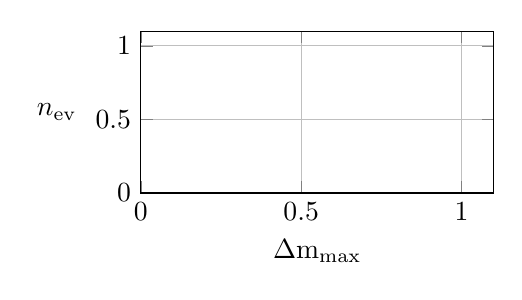
\begin{tikzpicture}[]
    \begin{axis}[height = {0.3\textwidth}, legend pos = {north east}, ymin = {0}, xmin = {0}, width = {0.5\textwidth},
      ylabel=$n_{\rm ev}$, ylabel style={rotate=-90}, xlabel=$\Delta {\rm m}_{\max}$, grid]
    \plotsol{fast}{rgb,1:red,1.00000000;green,0.000000000;blue,0.00000000}{nfev}{multipleshoot}{delta}
    \plotsol{interm}{rgb,1:red,0.00000000;green,0.50196078;blue,0.00000000}{nfev}{multipleshoot}{delta}
    \plotsol{slow}{rgb,1:red,0.00000000;green,0.000000000;blue,1.00000000}{nfev}{multipleshoot}{delta}
  \end{axis}
\end{tikzpicture}}
\subfloat[][]{
  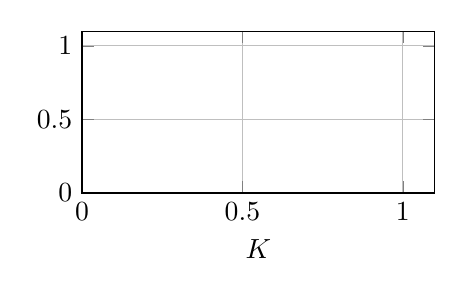
\begin{tikzpicture}[]
    \begin{axis}[height = {0.3\textwidth}, legend pos = {north east}, ymin = {0}, xmin = {0}, width = {0.5\textwidth},
      xlabel=$K$, grid]
    \plotsol{fast}{rgb,1:red,1.00000000;green,0.000000000;blue,0.00000000}{nfev}{multistage}{K}
    \plotsol{interm}{rgb,1:red,0.00000000;green,0.50196078;blue,0.00000000}{nfev}{multistage}{K}
    \plotsol{slow}{rgb,1:red,0.00000000;green,0.000000000;blue,1.00000000}{nfev}{multistage}{K}
  \end{axis}
  \end{tikzpicture}}
\caption{blabal}
\end{figure}
\end{document}